%% Based on <bare_jrnl.tex> in the ieee package available from CTAN,
%% I have changed the options so that most useful ones are clubbed together,
%% Have a look at <bare_jrnl.tex> to understand the function of each package. 

%% This code is offered as-is - no warranty - user assumes all risk.
%% Free to use, distribute and modify.

% *** Authors should verify (and, if needed, correct) their LaTeX system  ***
% *** with the testflow diagnostic prior to trusting their LaTeX platform ***
% *** with production work. IEEE's font choices can trigger bugs that do  ***
% *** not appear when using other class files.                            ***
% Testflow can be obtained at:
% http://www.ctan.org/tex-archive/macros/latex/contrib/supported/IEEEtran/testflow

%        File: pwe_3.tex
%     Created: Wed May 15 10:00  2019 S
% Last Change: Wed May 15 10:00  2019 S
%
\documentclass[journal]{IEEEtran}

\usepackage{cite, graphicx, amsmath} 
\usepackage[caption=false, font=footnotesize]{subfig}
\interdisplaylinepenalty=2500

% *** Do not adjust lengths that control margins, column widths, etc. ***
% *** Do not use packages that alter fonts (such as pslatex).         ***
% There should be no need to do such things with IEEEtran.cls V1.6 and later.




\begin{document}
%
% paper title
\title{Power Electronics Practical 3: Thyristors}
%
%
% author names and IEEE memberships
% note positions of commas and nonbreaking spaces ( ~ ) LaTeX will not break
% a structure at a ~ so this keeps an author's name from being broken across
% two lines.
% use \thanks{} to gain access to the first footnote area
% a separate \thanks must be used for each paragraph as LaTeX2e's \thanks
% was not built to handle multiple paragraphs
\author{R. de Bruyn, 216054484 \and Q. Kruger, 216008466}
%
% The paper headers
\markboth{University of Johannesburg}{University of Johannesburg}
% The only time the second header will appear is for the odd numbered pages
% after the title page when using the twoside option.


% If you want to put a publisher's ID mark on the page
% (can leave text blank if you just want to see how the
% text height on the first page will be reduced by IEEE)
%\pubid{0000--0000/00\$00.00~\copyright~2002 IEEE}

% use only for invited papers
%\specialpapernotice{(Invited Paper)}

% make the title area
\maketitle


\begin{abstract}
	A circuit using an SCR thyristor was implemented. The gate of the SCR
	was biased with a potentiometer which allows the firing angle of the
	SCR to be changed in the context of an AC input signal.
\end{abstract}

\section{Aim}

The aim of this experiment is to create a circuit which shows the operation of
an SRC type thyristor and to briefly explain and show the concept of holding
current and latching current.

\section{Circuit and Results}

The circuit was primarily a resistive circuit, as shown below. The oscillograms
obtained by testing the circuit are shown in Figure \ref{fig:results}.

\begin{figure}[h]
	\centering
	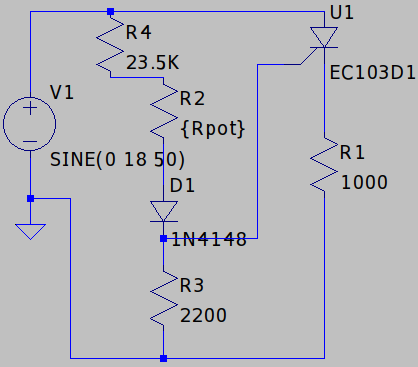
\includegraphics[width=.6\linewidth]{./img/circuit.png}
	\caption{Circuit diagram}
	\label{fig:circuit}
\end{figure}

\begin{figure}
	\centering
	\subfloat[Firing angle $\alpha_1$\label{fig:a}]{
		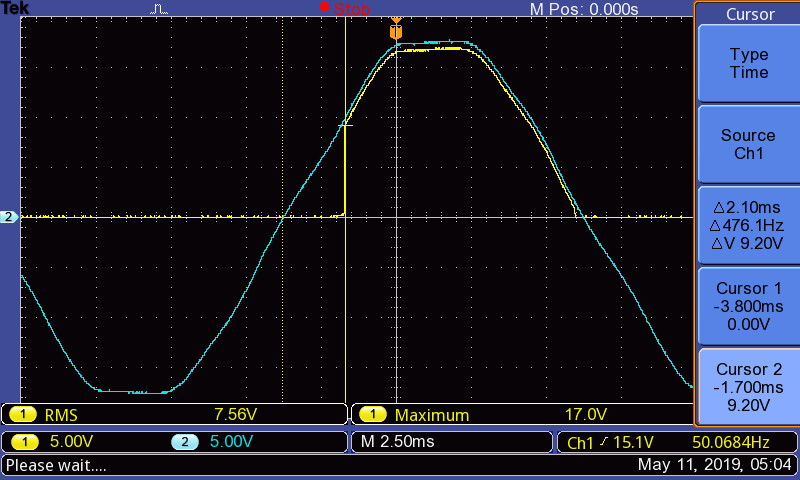
\includegraphics[width=\linewidth]{./img/TEK0004.jpg}
	}

	\subfloat[Firing angle $\alpha_2$\label{fig:b}]{
		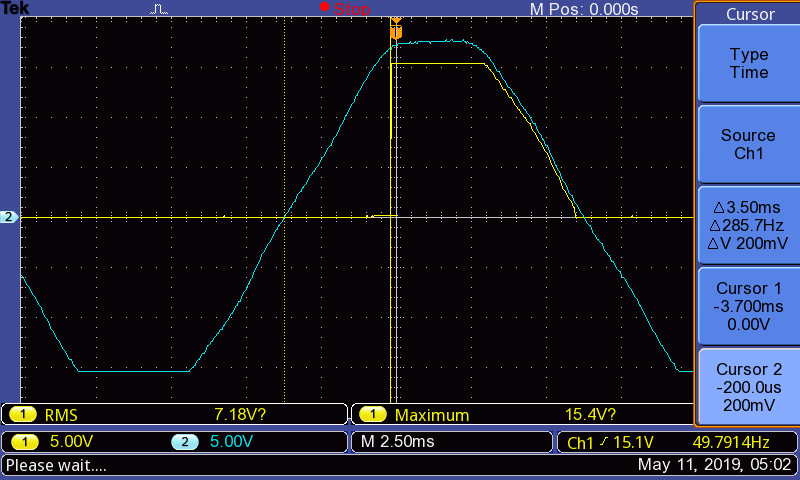
\includegraphics[width=\linewidth]{./img/TEK0003.jpg}
	}

	\caption{Results showing different firing angles}
	\label{fig:results}
\end{figure}

The input voltage was a 50Hz AC signal with 18V peak, which implies a period of
20ms. Thus, a firing delay of 10ms corresponds to a firing angle of 180 degrees.
From Figure \ref{fig:a} we can see that we have a firing angle of

\begin{equation}
	\alpha_1 = \frac{2.1 \times 10^{-3}}{10 \times 10^{-3}} 180^\circ = 37.8^\circ
	\label{eq:alpha_1}
\end{equation}

and, by adjusting the potentiometer to provide a larger resistance, the firing
angle from Figure \ref{fig:b} yields a firing angle of

\begin{equation}
	\alpha_2 = \frac{3.5 \times 10^{-3}}{10 \times 10^{-3}} 180^\circ = 63^\circ
	\label{eq:alpha_2}
\end{equation}

\section{Discussion and Conclusion}

The datasheet of our EO102AB SCR \cite{scr_datasheet} yields an approximate gate
latching current of $200\mu$A. \textit{Latching current} is the current at
which the thyristor switches on in forward-blocking mode. Our circuit was
designed to bias the gate of the thyristor, delaying the latching current of
$200\mu$A to adjust the firing angle.

The concept of \textit{holding current} is that, since a thyristor can be
modeled as a PNP transistor feeding the base of an NPN transistor, the current
through the collector of the PNP transistor needs to be enough to keep the NPN
transistor biased in saturation mode (i.e to act as a switch). When the holding
current is less than a certain threshold, the NPN transistor starts operating
downwards in its amplifying region, letting less current from the source into
its collector. This in turn causes the PNP to pass less current through its
base. This effect continues until both transistors essentially switch each
other off.

We also saw that the firing angle from cannot be more than $90^\circ$,
otherwise the SCR never switches on. This makes sense, because in this case the
peak current is less than the latching current, making it impossible to switch
the SCR on in this state.

% needed in second column of first page if using \pubid
%\pubidadjcol

% trigger a \newpage just before the given reference
% number - used to balance the columns on the last page
% adjust value as needed - may need to be readjusted if
% the document is modified later
%\IEEEtriggeratref{8}
% The "triggered" command can be changed if desired:
%\IEEEtriggercmd{\enlargethispage{-5in}}

% references section

%\bibliographystyle{IEEEtran.bst}
%\bibliography{IEEEabrv,../bib/paper}
\begin{thebibliography}{1}

	\bibitem{scr_datasheet}
		EO102AB SCR datasheet, \textit{www.chipdocs.com/datasheets/datasheet-pdf/TAG/E0102.html}

\end{thebibliography}

\end{document}


